\documentclass[envcountsect, 10pt, portrait, palatino]{beamer}
\usepackage{verbatim}
\usepackage{amsmath}
\usepackage{color}
\usepackage{listings}
%%%%%%%%%%%%%%%%%%%%%%%%%%%%%%% Beamer packages %%%%%%%%%%%%%%%%%%%%%%%
\usetheme{CambridgeUS}
\usefonttheme[onlylarge]{structurebold}
\setbeamerfont*{frametitle}{size=\normalsize,series=\bfseries}
\setbeamertemplate{navigation symbols}{}

\mode<presentation>{
% XXX without this the number does not appear
%\AtBeginDocument{\def\figurename{{\scshape Figure~\thesection.\thefigure}}}
}
% to number captions
\setbeamertemplate{theorems}[ams style]
\setbeamertemplate{caption}[numbered]
%\setbeamertemplate{theorems}[numbered]
%%%%%%%%%%%%%%%%%%%%%%%%%%%% title slide %%%%%%%%%%%%%%%%%%%%%%%%%%%%%%
\title[]{Applied survival analysis}
\author[Constantin T Yiannoutsos]
{ Constantin T Yiannoutsos, Ph.D.}

\date[]{\today}
\newtheorem{defn}{Definition}[section]
\newtheorem{assu}[defn]{Assumption}
\newcommand{\simdot}{\stackrel{\cdot}{\sim}}
\newcommand{\bfbeta}{{\mbox{\boldmath$\beta$}}}
\newcommand{\bfep}{{\mbox{\boldmath$\epsilon$}}}
\newcommand{\bhat}{\hat{\beta}}
\newcommand{\btilde}{\tilde{\mbox{\boldmath$\beta$}}}
\newcommand{\bfmu}{{\mbox{\boldmath$\mu$}}}
\newcommand{\Var}{{\rm Var}}
\newcommand{\Cov}{{\rm Cov}}
\newcommand{\trt}{{\rm trt}}
\newcommand{\pr}{{\rm pr}}
\newcommand{\age}{{\rm age}}
\newcommand{\Sin}{\sum_{i=1}^N}
\newcommand{\Sjn}{\sum_{j=1}^N}
\newcommand{\ui}{{\bf u}_i}
\newcommand{\uj}{{\bf u}_j}
\newcommand{\bfx}{{\mbox{{\bf x}}}}
\newcommand{\bfp}{{\mbox{{\bf p}}}}
\newcommand{\hbfp}{\widehat{\mbox{{\bf p}}}}
\newcommand{\bfy}{{\mbox{{\bf y}}}}
\newcommand{\bfY}{{\mbox{{\bf Y}}}}
\newcommand{\bfZ}{{\mbox{{\bf Z}}}}
\newcommand{\bfa}{{\mbox{{\bf a}}}}
\newcommand{\bfb}{{\mbox{{\bf b}}}}
\newcommand{\bfg}{{\mbox{{\bf g}}}}
\newcommand{\bfU}{{\bf U}}
\newcommand{\bfu}{{\mbox{{\bf u}}}}
\newcommand{\bfz}{{\mbox{{\bf z}}}}
\newcommand{\logit}{{\mbox{{logit}}}}
\newcommand{\bfzero}{{\mbox{{\bf 0}}}}
\newcommand{\hbeta}{{\widehat \beta}}
\newcommand{\heta}{{\widehat \eta}}
\newcommand{\hsigma}{{\widehat \sigma}}
\newcommand{\hmu}{{\widehat \mu}}
\newcommand{\hpi}{{\widehat \pi}}
\newcommand{\cI}{{\cal I}}
\newcommand{\bsigma}{{\bar \sigma}}
\newcommand{\brho}{{\bar \rho}}
\newcommand{\bx}{ {\bar {x} } }
\newcommand{\bY}{ {\bar {Y} } }
\newcommand{\hY}{ {\widehat {Y} } }
\newcommand{\hp}{ {\widehat {p} } }
\newcommand{\hVar}{ {\widehat {Var} } }
\newcommand{\bfI}{\mathbf{I}}

\setlength{\baselineskip}{2.5em}
% The main document
\begin{document}
\begin{frame}
  \titlepage
\end{frame}
%%%%%%%%%%%%%%%%%%%%%%%%%%%%%%%%%%%%%%%%%%%%%%%%%%%%%%%%%%%%%%%%%%%%%%%
\begin{frame}{Contents of today's lecture}
  \tableofcontents
\end{frame}
\section{ Parametric Survival Analysis}
\subsection{Introduction}
\begin{frame}{Parametric survival analysis}

So far, we have focused primarily on nonparametric and
semi-parametric approaches to survival analysis, with heavy
emphasis on the Cox proportional hazards model:
\begin{eqnarray*}
\lambda(t,\bfZ) & = & \lambda_0(t) ~ \exp(\bfbeta \bfZ)
\end{eqnarray*}

We used the following estimating approach:
\begin{itemize}
\item We estimated $\lambda_0(t)$ nonparametrically,
using the Kaplan-Meier estimator, or using the
Kalbfleisch/Prentice estimator under the PH assumption
\item We estimated $\bfbeta$ by assuming a linear model
between the log HR and covariates, under the PH model
\end{itemize}
Both estimates were based on maximum likelihood theory.
\\[2ex]
\underline{\bf Reading:} for parametric models see Collett.
%%%%%%%%%%%%%%%%%%%%%%%%%%%%%%%%%%%%%%%%%%%%%%%%%%%%%%%%%%%%%%%%
\end{frame}
\begin{frame}{Reasons for considering a parametric approach}
There are several reasons why we should consider some
alternative approaches based on parametric models:

\begin{itemize}
\item  The assumption of proportional hazards might not be \\
appropriate (based on major departures)
\item  If a parametric model actually holds, then we would probably
gain efficiency
\item  We may want to handle non-standard situations like
\begin{itemize}
\item  interval censoring
\item  incorporating population mortality
\end{itemize}
\item  We may want to make some connections with other
familiar approaches
 (e.g. use of the Poisson likelihood)
\item We may want to obtain some estimates for use in designing a
future survival study.
\end{itemize}
\end{frame} 
\subsection{Exponential regression}
\begin{frame}{A simple start:  Exponential Regression}

\begin{itemize}
\item \underline{\bf Observed data:} ~~~$(X_i, \delta_i, {\bf Z}_i)$
for individual $i$,\\
~~~~~$\bfZ_i= (Z_{i1}, Z_{i2},...,Z_{ip})$ represents a set of $p$
covariates.\\
\item {\bf Right censoring:}  Assume that  $X_i = \min(T_i,U_i)$\\
\item {\bf Survival distribution:} Assume $T_i$ follows an exponential
distribution with a parameter $\lambda$ that depends on $\bfZ_i$,
say $\lambda_i=\Psi(\bfZ_i)$.  Then we can write:
\[  T_i \sim exponential(\Psi(\bfZ_i)) \]
\end{itemize}

\end{frame} 
\begin{frame}{Review}
First, let's review some facts about the exponential distribution
(from our first survival lecture):
\begin{eqnarray*}
f(t) & = & \lambda e^{-\lambda t} ~~~~~~~~~\mbox{ for } t\ge 0 \\[2ex]
S(t) & = & P(T \geq t) = \int_t^\infty f(u) du = e^{-\lambda t} \\[2ex]
F(t) & = & P(T < t) = 1 - e^{-\lambda t} \\[2ex]
\lambda(t) & = & \frac{f(t)}{S(t)} =  \lambda
~~~~~\mbox{ constant hazard!} \\[2ex]
\Lambda(t) & = & \int_0^t \lambda(u) \, du  =  \int_0^t \lambda \, du
= \lambda t
\end{eqnarray*}
%%%%%%%%%%%%%%%%%%%%%%%%%%%%%%%%%%%%%%%%%%%%%%%%%%%%%%%%%%%%%%%%
\end{frame} 
\begin{frame}{Modeling the hazard in exponential regression}
Now, we say that $\lambda$ is a constant {\em over time} $t$, but we
want to let it depend on the covariate values, so we are setting
\begin{eqnarray*}
\lambda_i & = & \Psi(\bfZ_i)
\end{eqnarray*}

The hazard rate would therefore be the same for any two individuals
with the same covariate values.

Although there are many possible choices for $\Psi$, one simple and
natural choice is:
\[\Psi(\bfZ_i) =
\exp[ \beta_0 + Z_{i1} \beta_1 + Z_{i2} \beta_2 + ... + Z_{ip} \beta_p] \]

{\bf WHY?}
\begin{itemize}
\item ensures a positive hazard
\item for an individual with ${\bfZ}={\bf 0}$, the hazard is
$e^{\beta_0}$.
\end{itemize}
The model is called {\bf exponential regression} because of
the natural generalization from regular linear regression
%%%%%%%%%%%%%%%%%%%%%%%%%%%%%%%%%%%%%%%%%%%%%%%%%%%%%%%%%%%%%%%%
\end{frame} 
\begin{frame}{Exponential regression for the 2-sample case}

\begin{itemize}
\item Assume we have only a single covariate $\bfZ=Z$,\\
i.e., ($p=1$).\\

\underline{\bf Hazard Rate:}
\[\Psi(\bfZ_i) = \exp( \beta_0 + Z_i \beta_1 ) \]

\item Define:~~~~
\begin{tabular}{ll}
$Z_{i}= 0$  & if individual $i$ is in group 0\\
$Z_{i}= 1$  & if individual $i$ is in group 1\\
\end{tabular}

\item {\bf What is the hazard for group 0?}
%the hazard for group 0 is $\lambda_0=e^{\beta_0}$
\item {\bf What is the hazard for group 1?}
%the hazard for group 1 is $\lambda_1=e^{\beta_0+\beta_1} $
\item {\bf What is the hazard ratio of group 1 to group 0?}
% the hazard ratio is $\frac{\lambda_1}{\lambda_0} = e^{\beta_1}$
\item {\bf What is the interpretation of $\beta_1$?}
\end{itemize}
%%%%%%%%%%%%%%%%%%%%%%%%%%%%%%%%%%%%%%%%%%%%%%%%%%%%%%%%%%%%%%%%
\end{frame} 
\begin{frame}{Likelihood for Exponential Model}

Under the assumption of right censored data, each person has one of
two possible contributions to the likelihood:
\begin{itemize}
\item[(a)] they have an {\bf event} at $X_i$ ($\delta_i=1$) $\Rightarrow$
contribution is
\begin{eqnarray*}
L_i & = & \underbrace{~~~~S(X_i)~~~~}
~ \cdot ~ \underbrace{~~~\lambda(X_i)~~~}
~=~ e^{-\lambda X_i} ~ \lambda\\[1ex]
    &   & \mbox{survive to $X_i$} ~~~~~ \mbox{fail at $X_i$}
\end{eqnarray*}

\item[(b)] they are {\bf censored} at $X_i$ ($\delta_i=0$) $\Rightarrow$
contribution is
\begin{eqnarray*}
L_i & = & \underbrace{~~~~S(X_i)~~~~} ~=~ e^{-\lambda X_i}\\[1ex]
    &   & \mbox{survive to $X_i$}
\end{eqnarray*}
\end{itemize}
\end{frame}
\begin{frame}{The likelihood for the exponential model (cont'd)}
The {\bf likelihood} is the product over all of the individuals:
\begin{eqnarray*}
{\cal L} & = & \prod_i ~ L_i \\
& = & \prod_i ~\underbrace{\left(\lambda e^{-\lambda X_i}\right)^{\delta_i}}
  ~~ \underbrace{\left(e^{-\lambda X_i}\right)^{(1-\delta_i)}}\\
& & ~~~~~~~~\mbox{events} ~~~~~~~ \mbox{censorings}\\[2ex]
         & = & \prod_i ~\lambda^{\delta_i} ~\left(e^{-\lambda X_i}\right)
\end{eqnarray*}
%%%%%%%%%%%%%%%%%%%%%%%%%%%%%%%%%%%%%%%%%%%%%%%%%%%%%%%%%%%%%%%%
\end{frame} 
\begin{frame}{Maximum Likelihood for Exponential}

\vspace{0.3in}
{\bf How do we use the likelihood?}
\begin{itemize}
\item first take the log
\item then take the partial derivative with respect to $\bfbeta$
\item then set to zero and solve for $\widehat\bfbeta$
\item this gives us the {\bf maximum likelihood estimators}
\end{itemize}
\end{frame}
\begin{frame}{Likelihood equations}
The log-likelihood is:
\begin{eqnarray*}
\log {\cal L} & = &
\log \left[\prod_i ~
\lambda^{\delta_i} ~~\left(e^{-\lambda X_i}\right)\right]\\[2ex]
& = & \sum_i \left[\delta_i \log(\lambda) - \lambda X_i\right]\\[2ex]
& = & \sum_i \left[\delta_i \log(\lambda)\right] - \sum_i \lambda X_i
\end{eqnarray*}
For the case of exponential regression, we now substitute the
hazard $\lambda=\Psi(\bfZ_i)$ in the above log-likelihood:
\begin{eqnarray}
\log {\cal L} & = &
\sum_i \left[\delta_i \log(\Psi(\bfZ_i))\right] - \sum_i \Psi(\bfZ_i) X_i
\label{loglik}
\end{eqnarray}
%%%%%%%%%%%%%%%%%%%%%%%%%%%%%%%%%%%%%%%%%%%%%%%%%%%%%%%%%%%%%%%%
\end{frame} 
\begin{frame}{General Form of Log-likelihood for Right Censored Data}

In general, whenever we have right censored data, the likelihood and
corresponding log likelihood will have the following forms:
\begin{eqnarray*}
{\cal L} & = &\prod_i \left[\lambda_i(X_i)\right]^{\delta_i} \, S_i(X_i)\\
\log {\cal L} & = &
\sum_i \left[\delta_i \log{(\lambda_i(X_i))}\right] - \sum_i \Lambda_i(X_i)
\end{eqnarray*}
where
\begin{itemize}
\item $\lambda_i(X_i)$ is the hazard for the individual $i$ who
fails at $X_i$
\item $\Lambda_i(X_i)$ is the cumulative hazard for an individual
at their failure \underline{or} censoring time
\end{itemize}
For example, see the derivation of the likelihood for a Cox model on
p.11-18 of Lecture 4 notes.  We started with the likelihood above,
then substituted the specific forms for $\lambda(X_i)$ under the PH
assumption.
%%%%%%%%%%%%%%%%%%%%%%%%%%%%%%%%%%%%%%%%%%%%%%%%%%%%%%%%%%%%%%%%
\end{frame} 
\begin{frame}
Consider our model for the hazard rate:
\[\lambda = \Psi(\bfZ_i) =
\exp[ \beta_0 + Z_{i1} \beta_1 + Z_{i2} \beta_2 + ... + Z_{ip} \beta_p] \]

We can write this using vector notation, as follows:
\begin{eqnarray*}
\mbox{Let~~~} \bfZ_i & = & (1,Z_{i1},...Z_{ip})^T \\[1ex]
\mbox{and~~~} \bfbeta & = & (\beta_0, \beta_1,...\beta_p)
\end{eqnarray*}

(Since $\beta_0$ is the intercept (i.e., the log hazard rate for
the baseline group), we put a ``1'' as the first term in the vector
$\bfZ_i$.) Then, we can write the hazard as:
\[    \Psi(\bfZ_i) =   \exp[ \bfbeta \bfZ_i ] \]
Now we can substitute $\Psi(\bfZ_i) = \exp[\bfbeta \bfZ_i]$ in the
log-likelihood shown in (\ref{loglik}):
\begin{eqnarray*}
\log {\cal L} & = &
\sum_{i=1}^{n} {\delta_i} (\bfbeta \bfZ_i) -
\sum_{i=1}^{n} X_i\exp( \bfbeta \bfZ_i )
\end{eqnarray*}
%%%%%%%%%%%%%%%%%%%%%%%%%%%%%%%%%%%%%%%%%%%%%%%%%%%%%%%%%%%%%%%%
\end{frame} 
\begin{frame}{Score Equations}

Taking the derivative with respect to $\beta_0$, the
score equation is:
\begin{eqnarray*}
\frac{\partial\log{\cal L}}{\partial \beta_0}
& =  &  \sum_{i=1}^{n}  [ {\delta_i} - X_i \exp( \bfbeta \bfZ_i )]  \\
\end{eqnarray*}
For $\beta_k$, $k=1,...p$, the equations are:
\begin{eqnarray*}
\frac{\partial\log{\cal L}}{\partial \beta_k}   & =  &
\sum_{i=1}^{n} ~ [ {\delta_i} Z_{ik} - X_i Z_{ik} \exp( \bfbeta \bfZ_i )]\\
& =  &  \sum_{i=1}^{n} ~ Z_{ik} [{\delta_i} - X_i \exp( \bfbeta \bfZ_i )]
\end{eqnarray*}
To find the MLE's, we set the above equations to 0 and
solve (simultaneously).  The equations above imply that
the MLE's are obtained by setting the weighted number
of failures ($\sum_i Z_{ik} \delta_i$) equal to the weighted
cumulative hazard ($\sum_i Z_{ik} \Lambda(X_i)$).
%%%%%%%%%%%%%%%%%%%%%%%%%%%%%%%%%%%%%%%%%%%%%%%%%%%%%%%%%%%%%%%%
\end{frame} 
\begin{frame}{Variance of the MLE}
To find the variance of the MLE's, we need to take the
second derivatives:

\[ -~ \frac{\partial^2\log{\cal L}  }{\partial \beta_k \partial \beta_j}
=\sum_{i=1}^{n} Z_{ik}Z_{ij} X_i \exp( \bfbeta \bfZ_i )\]
Some algebra (see Cox and Oakes section 6.2) reveals that
\[ Var(\widehat{\bfbeta}) = I(\bfbeta)^{-1} =
\left[ \bfZ (\bfI-\Pi) \bfZ^T \right ]^{-1} \]
where
\begin{itemize}
\item $\bfZ=(\bfZ_1,\ldots,\bfZ_n)$ is a $(p+1)\times n$ matrix\\
($p$ covariates plus the ``1'' for the intercept $\beta_0$)

\item $\Pi=diag(\pi_1,\ldots,\pi_n)$ (this means that $\Pi$ is a
diagonal matrix, with the terms $\pi_1,\ldots,\pi_n$ on the diagonal)

\item $\pi_i$ is the probability that the $i$-{th} person is censored,
so $(1-\pi_i)$ is the probability that they failed.

\item  {\bf Note:} The information $I(\bfbeta)$ (inverse of the
variance) is proportional to the number of failures, not the sample
size.  This will be important when we talk about study design.
\end{itemize}
%%%%%%%%%%%%%%%%%%%%%%%%%%%%%%%%%%%%%%%%%%%%%%%%%%%%%%%%%%%%%%%%
\end{frame} 
\begin{frame}{The Single Sample Problem ($ Z_i = 1$ for everyone)}

First, what is the MLE of $\beta_0$?
\\[2ex]

We set  $\frac{\partial\log{\cal L}}{\partial
\beta_0}=\sum_{i=1}^{n}  [{\delta_i} - X_i \exp( \beta_0 Z_i )]$
equal to 0 and solve:
\begin{eqnarray*}
\Rightarrow ~~ \sum_{i=1}^{n} {\delta_i} & = &
\sum_{i=1}^{n} [X_i \exp(\beta_0)]\\
d & = & \exp(\beta_0) ~\sum_{i=1}^n X_i\\
\exp(\widehat{\beta_0}) & = & \frac{d}{\sum_{i=1}^n X_i}\\
\hat{\lambda} & = & \frac{d}{t}
\end{eqnarray*}
where $d$ is the total number of deaths (or events), and
$t=\sum X_i$ is the total person-time contributed by all individuals.
\end{frame} 
\begin{frame}{MLE estmate for $\beta$}
{\bf If $d/t$ is the MLE for $\lambda$, what does this imply about
the MLE of $\beta_0$?}
% MLE for beta_0 is log(d/t) or log d - log t
%%%%%%%%%%%%%%%%%%%%%%%%%%%%%%%%%%%%%%%%%%%%%%%%%%%%%%%%%%%%%%%%

Using the previous formula
$Var(\hat{\bfbeta}) = \left[ \bfZ (\bfI-\Pi) \bfZ^T \right]^{-1}$, \\
what is the variance of $\widehat{\beta}_0$?:

\vspace{0.3in}
With some matrix algebra, you can show that it is:

\begin{eqnarray*}
Var(\widehat{\beta}_0) & = & \frac{1}{\sum_{i=1}^n (1-\pi_i)} ~=~ \frac{1}{d}
\end{eqnarray*}

\end{frame} 
\begin{frame}{What about $\hat{\lambda} = e^{\hat{\beta}_0}$?}

By the delta method,
\begin{eqnarray*}
Var(\hat{\lambda}) & = & \hat\lambda^2 ~ Var(\widehat{\beta}_0)\\[3ex]
& = & ~~{\bf ?}
% = (d^2/t^2) (1/d) = d/t^2
\end{eqnarray*}
%%%%%%%%%%%%%%%%%%%%%%%%%%%%%%%%%%%%%%%%%%%%%%%%%%%%%%%%%%%%%%%%
\end{frame} \begin{frame}{The Two-Sample Problem:}

\begin{center}
\begin{tabular}{lcccc}
\hline
& $Z_i$ & Subjects & Events & Follow-up \\ \hline
{\bf Group 0:}~~
& $Z_{i}= 0$ & $n_0$ & $d_0$ & $t_0=\sum_{i=1}^{n_0} X_i$\\[1ex]
{\bf Group 1:}
& $Z_{i}= 1$ & $n_1$ & $d_1$ & $t_1=\sum_{i=1}^{n_1} X_i$ \\ \hline
\end{tabular}
\end{center}
\end{frame}
\begin{frame}{The log-likelihood}
\vspace{-0.3in}
\begin{eqnarray*}
\log {\cal L} & = &  \sum_{i=1}^{n} {\delta_i} (\beta_0 + \beta_1 Z_i) -
\sum_{i=1}^{n} X_i\exp(\beta_0 + \beta_1 Z_i)\\[2.5ex]
\mbox{so} ~~\frac{\partial\log{\cal L}  }{\partial \beta_0}
    & =  &  \sum_{i=1}^{n}  [ \delta_i -
   X_i \exp( \beta_0 + \beta_1 Z_{i} )]  \\[1ex]
   & =  & (d_0 + d_1) - (t_0 e^{\beta_0} + t_1 e^{\beta_0+\beta_1}) \\[2.5ex]
\frac{\partial\log{\cal L}  }{\partial \beta_1}
    & =  &  \sum_{i=1}^{n}  Z_i[ {\delta_i} -
   X_i \exp( \beta_0 + \beta_1 Z_{i} )]  \\[1ex]
   & =  &  d_1 -  t_1 e^{\beta_0+\beta_1}
\end{eqnarray*}
\end{frame}
\begin{frame}
\begin{eqnarray*}
\mbox{This implies:}~~~~~ \hat\lambda_1 & =
& e^{\hat{\beta_0} + \hat{\beta_1}} = ? \hspace{2in} \\[1.5ex]
% =d1/t1
\hat\lambda_0 & = & e^{\hat{\beta_0}} = ?\\[1.5ex]
% = d0/t0
\hat\beta_0 & = & ?\\[1.5ex]
% = log(d0/t0)
\hat\beta_1 & = & ?
% = log [(d1/t1) / (d0/t0)]
\end{eqnarray*}
%%%%%%%%%%%%%%%%%%%%%%%%%%%%%%%%%%%%%%%%%%%%%%%%%%%%%%%%%%%%%%%%
%\end{frame} 
%\begin{frame}{ Important Result}
%\vspace*{1in}
\begin{quote}
{\bf The maximum likelihood estimates (MLE's) of the hazard rates
under the exponential model are the number of events divided by
the person-years of follow-up!}
\end{quote}
\\[2ex]
%\vspace{1in}
(this result will be relied on heavily when we discuss study design)
%%%%%%%%%%%%%%%%%%%%%%%%%%%%%%%%%%%%%%%%%%%%%%%%%%%%%%%%%%%%%%%%
\end{frame}
\begin{frame}{Regression: Means and Medians}

\underline{\bf Mean Survival Time}
~\\[1ex]
For the exponential distribution, $E(T)=1/\lambda$.
\begin{itemize}
\item {\bf Control Group:}
\begin{eqnarray*}
\overline{T}_0 & = & 1/\hat\lambda_0 ~=~ 1/\exp(\hat\beta_0)
\end{eqnarray*}

\item {\bf Treatment Group:}
\begin{eqnarray*}
\overline{T}_1 & = & 1/\hat\lambda_1 ~=~ 1/\exp(\hat\beta_0 + \hat\beta_1)
\end{eqnarray*}
\end{itemize}
\end{frame} 
\begin{frame}{Means and medians (cont'd)}
\underline{\bf Median Survival Time}\\[1ex]
This is the value $M$ at which $S(t)=e^{-\lambda t}=0.5$,
so $M = \mbox{median} = \frac{-\log(0.5)}{\lambda}$
\begin{itemize}
\item {\bf Control Group:}
\begin{eqnarray*}
\hat{M_0} & = & \frac{-\log(0.5)}{\hat\lambda_0} ~=~
 \frac{-\log(0.5)}{~\exp(\hat\beta_0)}
\end{eqnarray*}

\item {\bf Treatment Group:}
\begin{eqnarray*}
\hat{M_1} & = & \frac{-\log(0.5)}{\hat\lambda_1} ~=~
 \frac{-\log(0.5)}{~\exp(\hat\beta_0 + \hat\beta_1)}
\end{eqnarray*}
\end{itemize}
%%%%%%%%%%%%%%%%%%%%%%%%%%%%%%%%%%%%%%%%%%%%%%%%%%%%%%%%%%%%%%%%
\end{frame} 
\begin{frame}{Exponential Regression: Variance Estimates and Test Statistics}

We can also calculate the variances of the MLE's as simple
functions of the number of failures:
\begin{eqnarray*}
var(\hat\beta_0) & = & \frac{1}{d_0}\\[2ex]
var(\hat\beta_1) & = & \frac{1}{d_0} + \frac{1}{d_1}
\end{eqnarray*}
\end{frame} 
\begin{frame}{Inference}
So our test statistics are formed as:

\underline{\bf For testing $H_o: \beta_0=0$:}
\vspace*{-1em}
\begin{eqnarray*}
\chi^2_w & = & \frac{\left(\hat\beta_0\right)^2}{var(\hat\beta_0)}\\
         & = & \frac{[\log(d_0/t_0)]^2}{1/d_0}
\end{eqnarray*}
\underline{\bf For testing $H_o: \beta_1=0$:}
\begin{eqnarray*}
\chi^2_w & = & \frac{\left(\hat\beta_1\right)^2}{var(\hat\beta_1)}\\
         & = & \frac{\left[\log(\frac{d_1/t_1}{d_0/t_0})\right]^2}
{\frac{1}{d_0} + \frac{1}{d_1}}
\end{eqnarray*}
{\bf How would we form confidence intervals for the hazard ratio?}
%%%%%%%%%%%%%%%%%%%%%%%%%%%%%%%%%%%%%%%%%%%%%%%%%%%%%%%%%%%%%%%%
\end{frame}
\begin{frame}{The Likelihood Ratio test statistic}
This is an alternative to the Wald test. It is based on 2 times the log of the
ratio of the likelihoods under the null and alternative.
We reject  H$_0$ if 2 log(LR) $> \chi^2_{1,0.05}$, where

\[ LR  = \frac{{\cal L}(H_1)}{{\cal L}(H_0)}  =
\frac{{\cal L}(\widehat{\lambda}_0,\widehat{\lambda}_1)}
{{\cal L}(\widehat{\lambda})} \]
\end{frame} 
\begin{frame}{The Likelihood Ratio test statistic (cont'd)}
For a sample of $n$ independent exponential random
variables with parameter $\lambda$,  the  Likelihood is:\\
\begin{eqnarray*}
  L &  = &  \prod_{i=1}^{n} [\lambda^{\delta_i} \exp(-\lambda x_i)]\\
    &  = &  \lambda^{d} \exp(-\lambda \sum x_i)\\
    &  = &  \lambda^{d} \exp(-\lambda n \bar{x})
\end{eqnarray*}
where $d$ is the number of deaths or failures.  The  log-likelihood is
\[ \ell = d \log(\lambda)  - \lambda n \bar{x}\]
and the MLE is \[ \widehat{\lambda}=d/(n \bar{x})\]
%%%%%%%%%%%%%%%%%%%%%%%%%%%%%%%%%%%%%%%%%%%%%%%%%%%%%%%%%%%%%%%%
\end{frame} 
\begin{frame}{2-Sample Case:  LR test calculations}

\underline{\bf Data:}

\begin{tabular}{ll}
Group 0: ~~~ & $d_0$ failures among the $n_0$ females\\
             & mean failure time is $\bar{x}_0 = (\sum_i^{n_0} X_i)/n_0$\\[1ex]
Group 1: ~~~ & $d_1$ failures among the $n_1$ males\\
             & mean failure time is $\bar{x}_1 = (\sum_i^{n_1} X_i)/n_1$\\
\end{tabular}

\vspace{0.3in}
Under the \underline{\bf alternative hypothesis}:
\begin{eqnarray*}
{\cal L} & = & \lambda_1^{d_1} \exp(-\lambda_1 n_1 \bar{x}_1) \times
  \lambda_0^{d_0} \exp(-\lambda_0 n_0 \bar{x}_0)\\[1ex]
\log({\cal L}) & = &  d_1 \log(\lambda_1) - \lambda_1 n_1 \bar{x}_1 +
      d_0 \log(\lambda_0) - \lambda_0 n_0 \bar{x}_0
\end{eqnarray*}

The MLE's are:
\begin{eqnarray*}
\widehat{\lambda}_1 & = & d_1/(n_1 \bar{x}_1) \hspace{0.5in}
\mbox{for males}\\[1ex]
\widehat{\lambda}_0 & = & d_0/(n_0 \bar{x}_0) \hspace{0.5in}
\mbox{for females}
\end{eqnarray*}
\end{frame}
\begin{frame}{MLEs under the  \underline{\bf null hypothesis}}
\begin{eqnarray*}
{\cal L} & = &  \lambda^{d_1+d_0}
     \exp[-\lambda (n_1 \bar{x}_1 + n_0 \bar{x}_0)]\\[1ex]
\log({\cal L}) & = &  (d_1 + d_0) \log(\lambda) - \lambda [ n_1 \bar{x}_1 +
       n_0 \bar{x}_0]
\end{eqnarray*}

The corresponding MLE is
\[ \widehat{\lambda}=(d_1+d_0)/[n_1 \bar{x}_1 + n_0 \bar{x}_0]\]
%%%%%%%%%%%%%%%%%%%%%%%%%%%%%%%%%%%%%%%%%%%%%%%%%%%%%%%%%%%%%%%%
\end{frame} 
\begin{frame}{Constructing the LR test}
A likelihood ratio test can be constructed by taking twice
the difference of the log-likelihoods under the alternative
and the null hypotheses:

\[ -2 \left[ (d_0+d_1) \log \left(\frac{d_0+d_1}{t_0+t_1}\right) -
d_1 \log[d_1/t_1] - d_0 \log[d_0/t_0] \right] \]
\end{frame} 
\subsection{Exponential analysis of the nursing home example}
\begin{frame}{Nursing home example}
\underline{\bf For the females:}
\begin{itemize}
\item $n_0 = 1173$
\item $d_0 = 902$
\item $t_0 = 310754$
\item $\bar{x}_0 = 265 $
\end{itemize}

\underline{\bf For the males:}
\begin{itemize}
\item $n_1 = 418$
\item $d_1 = 367$
\item $t_1 = 75457$
\item $\bar{x}_1 = 181 $
\end{itemize}

Plugging these values in, we get a LR test statistic of 64.20.
%%%%%%%%%%%%%%%%%%%%%%%%%%%%%%%%%%%%%%%%%%%%%%%%%%%%%%%%%%%%%%%%
\end{frame} 
\begin{frame}{Hand Calculations using events and follow-up:}

By adding up ``{\sc los}'' for males to get $t_1$ and for
females to get $t_0$, I obtained:
\begin{itemize}
\item $d_0 = 902$ (females)\\
      $d_1 = 367$ (males)

\vspace{0.1in}
\item $t_0 = 310754$ (female follow-up)\\
      $t_1 = 75457$ (male follow-up)

\vspace{0.2in}
\
\item This yields an estimated log HR:
\begin{eqnarray*}
\hat\beta_1 & = & \log \left[ \frac{d1/t1}{d0/t0} \right]
= \log \left[ \frac{367/75457}{902/310754} \right]
= \log (1.6756) = 0.5162
\end{eqnarray*}
\end{itemize}
\end{frame}
\begin{frame}{Constructing the Wald test}
In the above calculations, the estimated standard error is:
\begin{eqnarray*}
\sqrt{var(\hat{\beta_1})} & = & \sqrt{\frac{1}{d_1} + \frac{1}{d_0}}
~=~ \sqrt{\frac{1}{902} + \frac{1}{367}}
~=~ 0.06192
\end{eqnarray*}
So the Wald test becomes:
\begin{eqnarray*}
\chi^2_W & = & \frac{\hat{\beta}_1^2}{var(\hat{\beta_1})}
 ~ = ~ \frac{(0.51619)^2}{0.061915} ~=~ 69.51
\end{eqnarray*}

\vspace{0.2in}
We can also calculate $\hat\beta_0= log(d_0/t_0) = -5.842$,\\
along with its standard error $se(\hat\beta_0)=\sqrt{(1/d0)} = 0.0333$
\end{frame} 
\subsection{R implementation of exponential regression}
\begin{frame}[fragile]{ Exponential Regression in R }

\scriptsize
\begin{verbatim}
Call:
survreg(formula = Surv(losyr, fail) ~ gender, data = nurshome,
    dist = "exp")
              Value Std. Error     z        p
(Intercept) -0.0578     0.0333 -1.73 8.28e-02
gender      -0.5162     0.0619 -8.34 7.62e-17

Scale fixed at 1

Exponential distribution
Loglik(model)= -1006.3   Loglik(intercept only)= -1038.4
	Chisq= 64.2 on 1 degrees of freedom, p= 1.1e-15
Number of Newton-Raphson Iterations: 5
n= 1591 
\end{verbatim}
\normalsize
Since $Z=8.337$, the chi-square test is $Z^2=69.51$.
%%%%%%%%%%%%%%%%%%%%%%%%%%%%%%%%%%%%%%%%%%%%%%%%%%%%%%%%%%%%%%%%
\end{frame} 
\subsection{The Weibull regression model}
\begin{frame}{The Weibull regression model}

At the beginning of the course, we saw that the survivorship function
for a Weibull random variable is:
\begin{eqnarray*}
 S(t) & = & \exp[- \lambda ( t^\kappa) ]
\end{eqnarray*}
and the hazard function is:
\begin{eqnarray*}
 \lambda(t) & = & \kappa \, \lambda \, t^{(\kappa-1)}
\end{eqnarray*}
The Weibull regression model assumes that for someone with
covariates ${\bfZ_i}$, the survivorship function is
\[  S(t; {\bfZ_i} ) = \exp[- \Psi(\bfZ_i)  ( t^\kappa) ] \]
where $\Psi(\bfZ_i)$ is defined as in exponential regression to be:
\[  \Psi(\bfZ_i)  = \exp[ \beta_0 +
      Z_{i1}  \beta_1 +  Z_{i2}  \beta_2  + ... Z_{ip}
    \beta_p] \]
For the 2-sample problem, we have:
\[  \Psi(\bfZ_i)  = \exp[ \beta_0 + Z_{i1}  \beta_1] \]
\end{frame} 
\begin{frame}{Weibull MLEs for the 2-sample problem:}

\underline{\bf Log-likelihood:}
\begin{eqnarray*}
\log {\cal L} & = &  \sum_{i=1}^{n} {\delta_i}
\log\left[\kappa \exp(\beta_0 + \beta_1 Z_i) X_i^{\kappa-1}\right] -
\sum_{i=1}^{n} X_i^{\kappa} \exp(\beta_0 +\beta_1 Z_i)
\end{eqnarray*}
\begin{eqnarray*}
\Rightarrow ~~~~ \exp(\hat\beta_0)  =  d_0/t_{0}\kappa ~~~~~
\exp(\hat\beta_0 + \hat\beta_1) = d_1/t_{1}\kappa
\end{eqnarray*}
where
\begin{eqnarray*}
t_{j\kappa}  =  \sum_{i=1}^{n_j} X_i^{\hat\kappa}
~~\mbox{among $n_j$ subjects}\\
\hat\lambda_0(t) = \hat\kappa ~\exp(\hat\beta_0) ~t^{\hat\kappa-1} \,\,\,
\hat\lambda_1(t) = \hat\kappa ~\exp(\hat\beta_0+\hat\beta_1)
~t^{\hat\kappa-1}
\end{eqnarray*}
\begin{eqnarray*}
     \widehat{HR} & = & \hat\lambda_1(t)/\hat\lambda_0(t)
= \exp(\hat\beta_1) \\
                  & = & \exp\left(\frac{d_1/t_{1}\kappa}
                       {d_0/t_{0}\kappa}\right)
\end{eqnarray*}
%%%%%%%%%%%%%%%%%%%%%%%%%%%%%%%%%%%%%%%%%%%%%%%%%%%%%%%%%%%%%%%%
\end{frame} 
\begin{frame}{Weibull Regression: Means and Medians}

\underline{\bf Mean Survival Time}\\[1ex]
For the Weibull distribution, $E(T)=\lambda^{(-1/\kappa)}
\Gamma[(1/\kappa) + 1]$.
\begin{itemize}
\item {\bf Control Group:}
\begin{eqnarray*}
\overline{T}_0 & = & \hat\lambda_0^{(-1/\hat\kappa)}~\Gamma[(1/\hat\kappa) + 1]
\end{eqnarray*}

\item {\bf Treatment Group:}
\begin{eqnarray*}
\overline{T}_1 & = & \hat\lambda_1^{(-1/\hat\kappa)}~\Gamma[(1/\hat\kappa) + 1]
\end{eqnarray*}
\end{itemize}

\end{frame} 
\begin{frame}{Median Survival Time}
For the Weibull distribution,
 $M = \mbox{median} = \left[\frac{-\log(0.5)}{\lambda}\right]^{1/\kappa}$
\begin{itemize}
\item {\bf Control Group:}
\begin{eqnarray*}
\hat{M_0} & = & \left[\frac{-\log(0.5)}{\hat\lambda_0}\right]^{1/\hat\kappa}
\end{eqnarray*}

\item {\bf Treatment Group:}
\begin{eqnarray*}
\hat{M_1} & = & \left[\frac{-\log(0.5)}{\hat\lambda_1}\right]^{1/\hat\kappa}
\end{eqnarray*}
\end{itemize}
where $\hat\lambda_0=\exp(\hat\beta_0)$ and
$\hat\lambda_1=\exp(\hat\beta_0+\hat\beta_1)$.
%%%%%%%%%%%%%%%%%%%%%%%%%%%%%%%%%%%%%%%%%%%%%%%%%%%%%%%%%%%%%%%%
\end{frame} 
\begin{frame}{The Gamma function}
Note:  the symbol $\Gamma$ is the ``gamma'' function.  If $x$ is an
integer, then
\begin{eqnarray*}
\Gamma(x) & = & (x-1)!
\end{eqnarray*}

In cases where $x$ is not an integer, this function has to be
evaluated numerically.  In homework and labs, I will supply this value
to you.

\vspace{0.4in}
The Weibull regression model is very easy to fit:
\begin{itemize}
\item In {\sc stata}:  Just specify {\tt dist(weibull)} instead \\
of {\tt dist(exp)} within the {\tt streg} command
\item In {\sc sas}: use model option {\tt dist=weibull} within the
{\tt proc lifereg} procedure
\item IN {\sc R}: we use the {\tt survreg } command with the {\tt dist="exp"} option.
\end{itemize}

Note: to get more information on these modeling procedures, use the
online help facilities.  
\end{frame} 
\subsection{Fitting the Weibull model in R}
\subsection{Weibull analysis of the nursing home example}
\begin{frame}[fragile]{Fitting the  Weibull  model in R}

\scriptsize
\begin{verbatim}
Call:
survreg(formula = Surv(losyr, fail) ~ gender, data = nurshome,
    dist = "weibull")
             Value Std. Error     z        p
(Intercept) -0.143     0.0542 -2.65 8.13e-03
gender      -0.673     0.1011 -6.66 2.67e-11
Log(scale)   0.487     0.0232 20.99 8.94e-98

Scale= 1.63

Weibull distribution
Loglik(model)= -731.1   Loglik(intercept only)= -751.9
	Chisq= 41.73 on 1 degrees of freedom, p= 1e-10
Number of Newton-Raphson Iterations: 5
n= 1591 
\end{verbatim}
\end{frame} 
\subsection{Goodness of fit}
\begin{frame}{Comparison of Exponential with Kaplan-Meier}

We can see how well the Exponential model fits by comparing
the survival estimates for males and females under the exponential
model, i.e., $P(T\ge t)=e^{(-\hat\lambda_z t)}$, to the Kaplan-Meier
survival estimates:
\\[-6ex]
\centerline{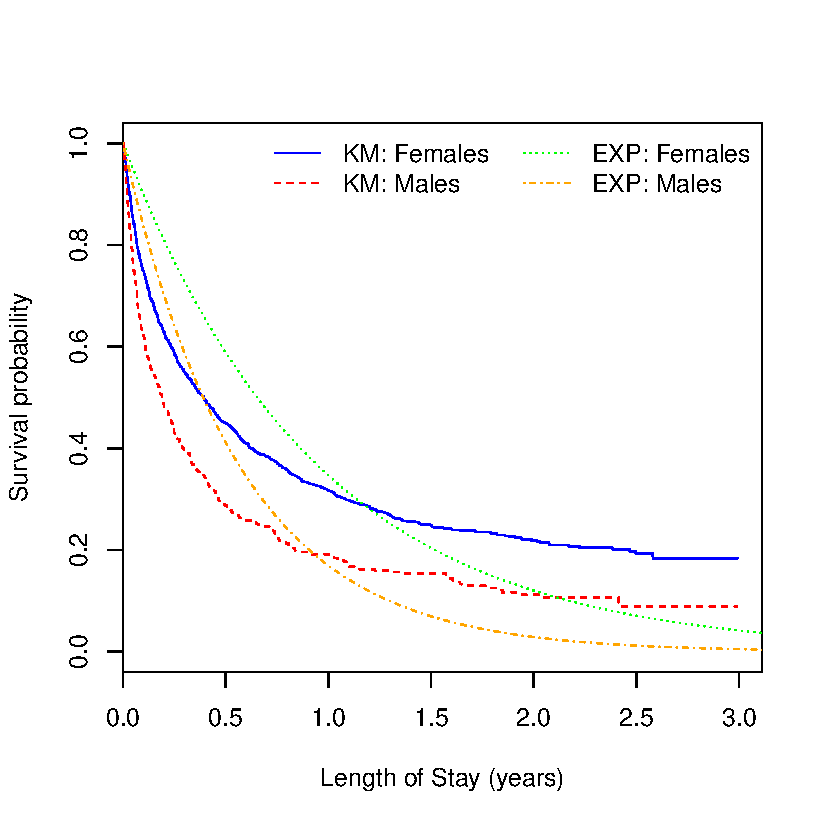
\includegraphics[width=3in]{ch12exp.pdf}}
%%%%%%%%%%%%%%%%%%%%%%%%%%%%%%%%%%%%%%%%%%%%%%%%%%%%%%%%%%%%%%%%
\end{frame} 
\begin{frame}{ Comparison of Weibull with Kaplan-Meier}

We can see how well the Weibull model fits by comparing
the survival estimates, $P(T\ge t)=e^{(-\hat\lambda_z t^{\hat\kappa})}$,
to the Kaplan-Meier survival estimates.\\[-4ex]
\centerline{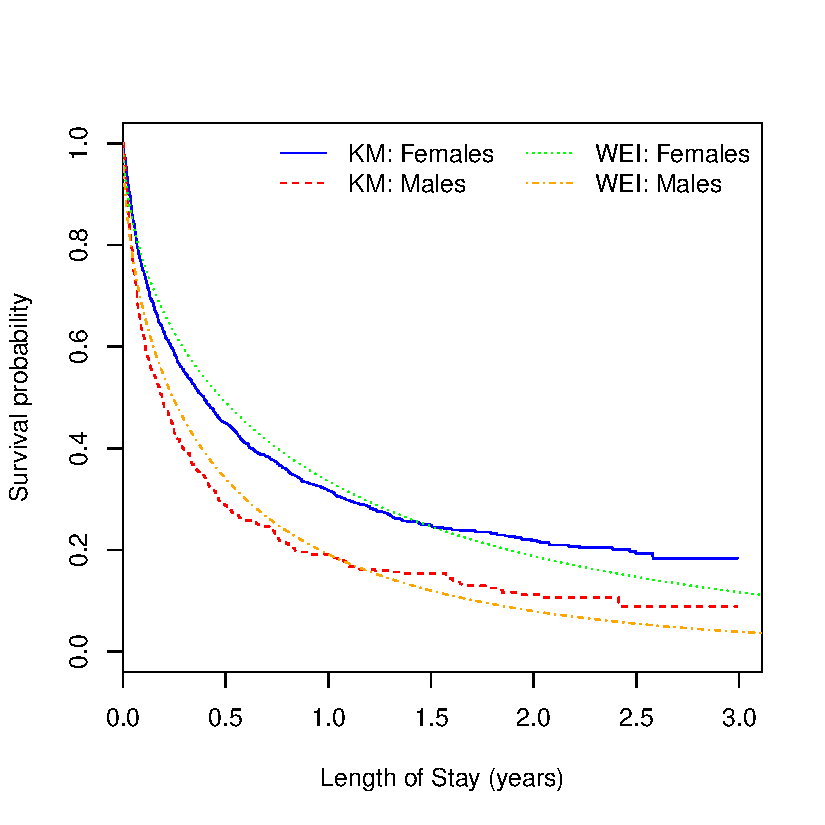
\includegraphics[width=3in]{ch12weib.pdf}}
{\bf Which do you think fits best?}
%%%%%%%%%%%%%%%%%%%%%%%%%%%%%%%%%%%%%%%%%%%%%%%%%%%%%%%%%%%%%%%%
\end{frame} 
\begin{frame}{Other useful plots for evaluating fit }
\begin{itemize}
\item  $-\log(\hat{S}(t))$ vs $t$

\vspace{0.2in}
\item  $\log[-\log(\hat{S}(t))]$ vs $\log(t)$
\end{itemize}

\vspace{0.2in}
Why are these useful?

{\bf If T is exponential}, then $S(t) = \exp(-\lambda t))$
\begin{eqnarray*}
\mbox{so}~~~~~ \log(S(t)) & = & -\lambda t\\
\mbox{and}~~~~~~~~~~ \Lambda(t) & = & \lambda \, t
\end{eqnarray*}

a straight line in $t$ with slope $\lambda$ and intercept=0\\[1ex]

\vspace{0.2in}
{\bf If T is Weibull}, then $S(t) = \exp(-(\lambda t)^\kappa)$
\begin{eqnarray*}
\mbox{so}~~~~~   \log(S(t)) & = & -\lambda t^\kappa\\
\mbox{then}~~~~~~~~~~~ \Lambda(t) & = &  \lambda t^\kappa\\
\mbox{and}~~~~~~  \log(-\log(S(t))) & = & \log(\lambda) + \kappa*\log(t)
\end{eqnarray*}

a straight line in $\log(t)$ with slope $\kappa$ and intercept $\log(\lambda)$.
%%%%%%%%%%%%%%%%%%%%%%%%%%%%%%%%%%%%%%%%%%%%%%%%%%%%
\end{frame} 
\begin{frame}{Goodness of fit plots}
So we can calculate our estimated $\Lambda(t)$ and plot it versus $t$,
and if it seems to form a straight line, then the exponential
distribution is probably appropriate for our dataset.

{\bf Plots for nursing home data: $\hat\Lambda(t)$ vs $t$}
\centerline{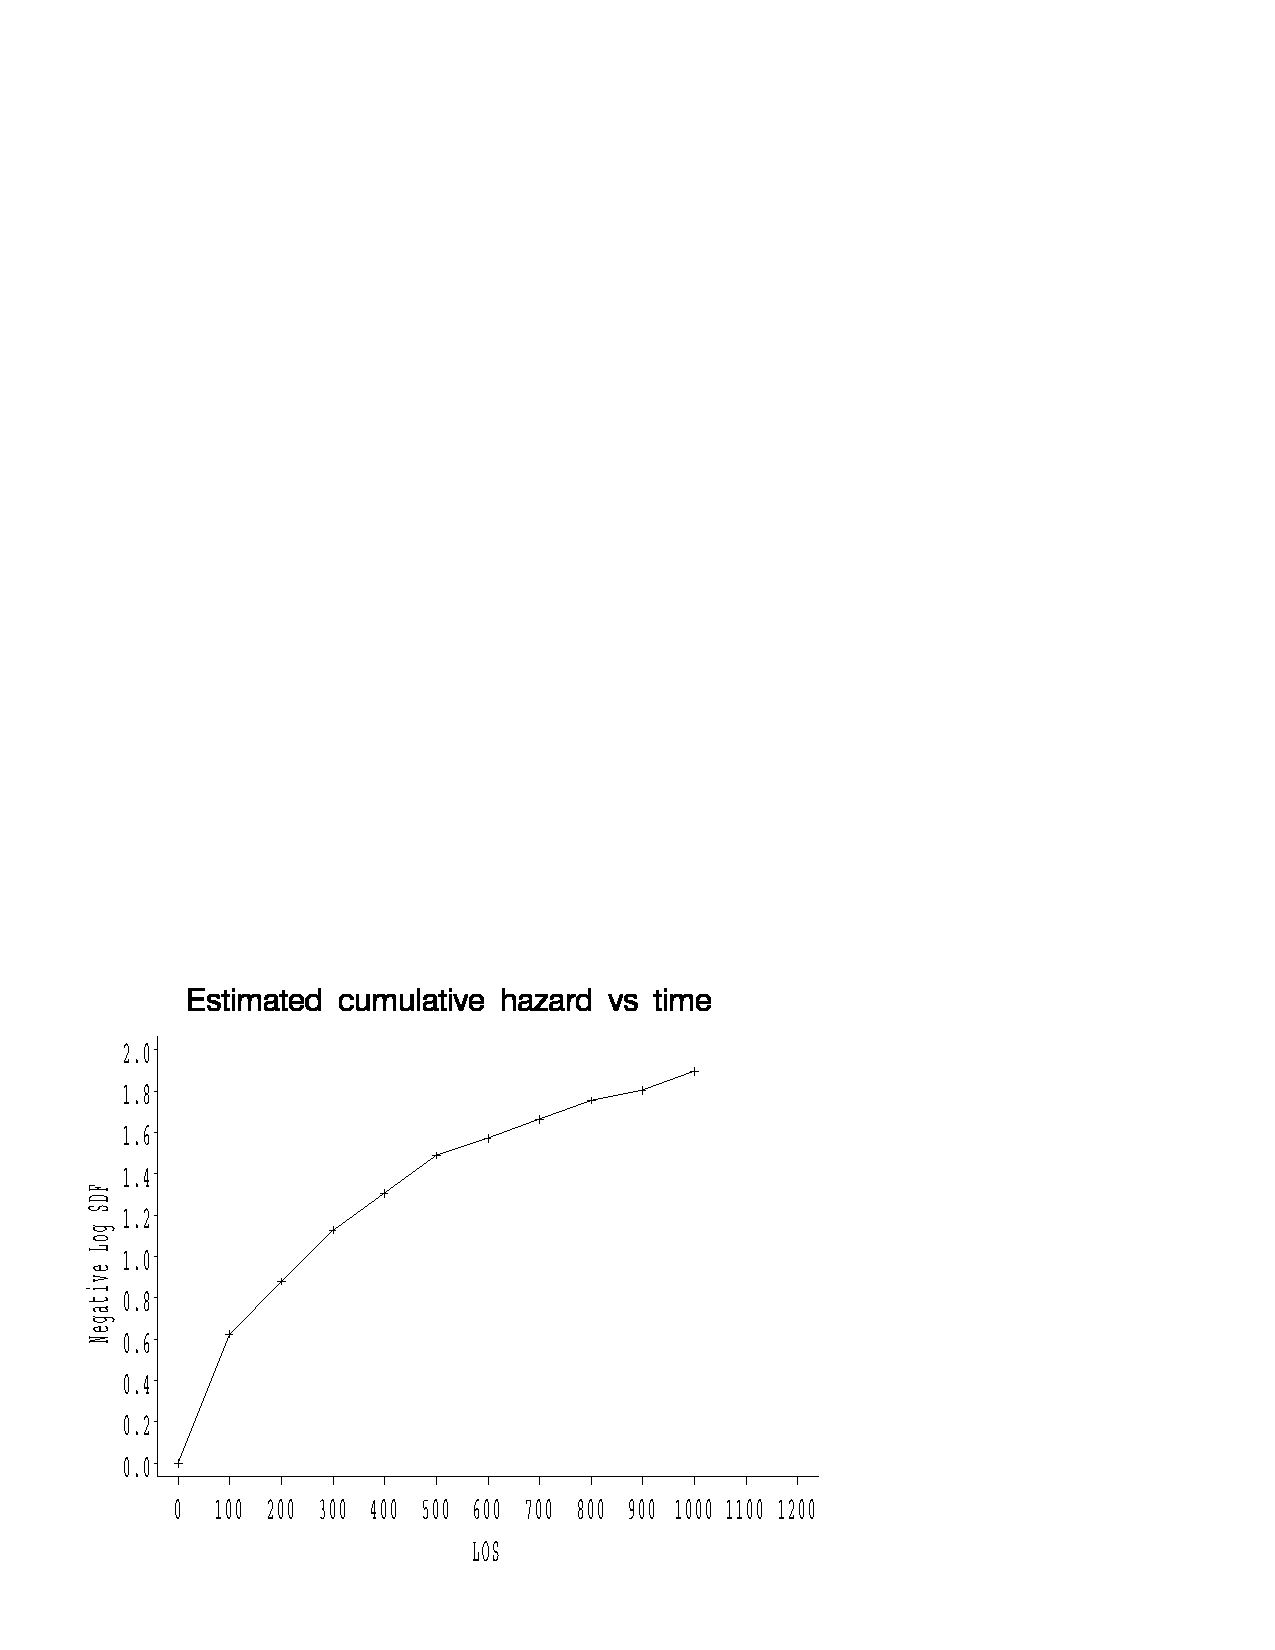
\includegraphics[width=3in]{nh_ls.pdf}}
%%%%%%%%%%%%%%%%%%%%%%%%%%%%%%%%%%%%%%%%%%%%%%%%%%%%
\end{frame} 
\begin{frame}{Log-log plot in the Weibull analysis}
Or we can plot $\log\hat\Lambda(t)$ versus $\log(t)$,
and if it seems to form a straight line, then the Weibull
distribution is probably appropriate for our dataset.

{\bf Plots for nursing home data: $\log[-log(\hat{S}(t))]$ vs $\log(t)$}

\centerline{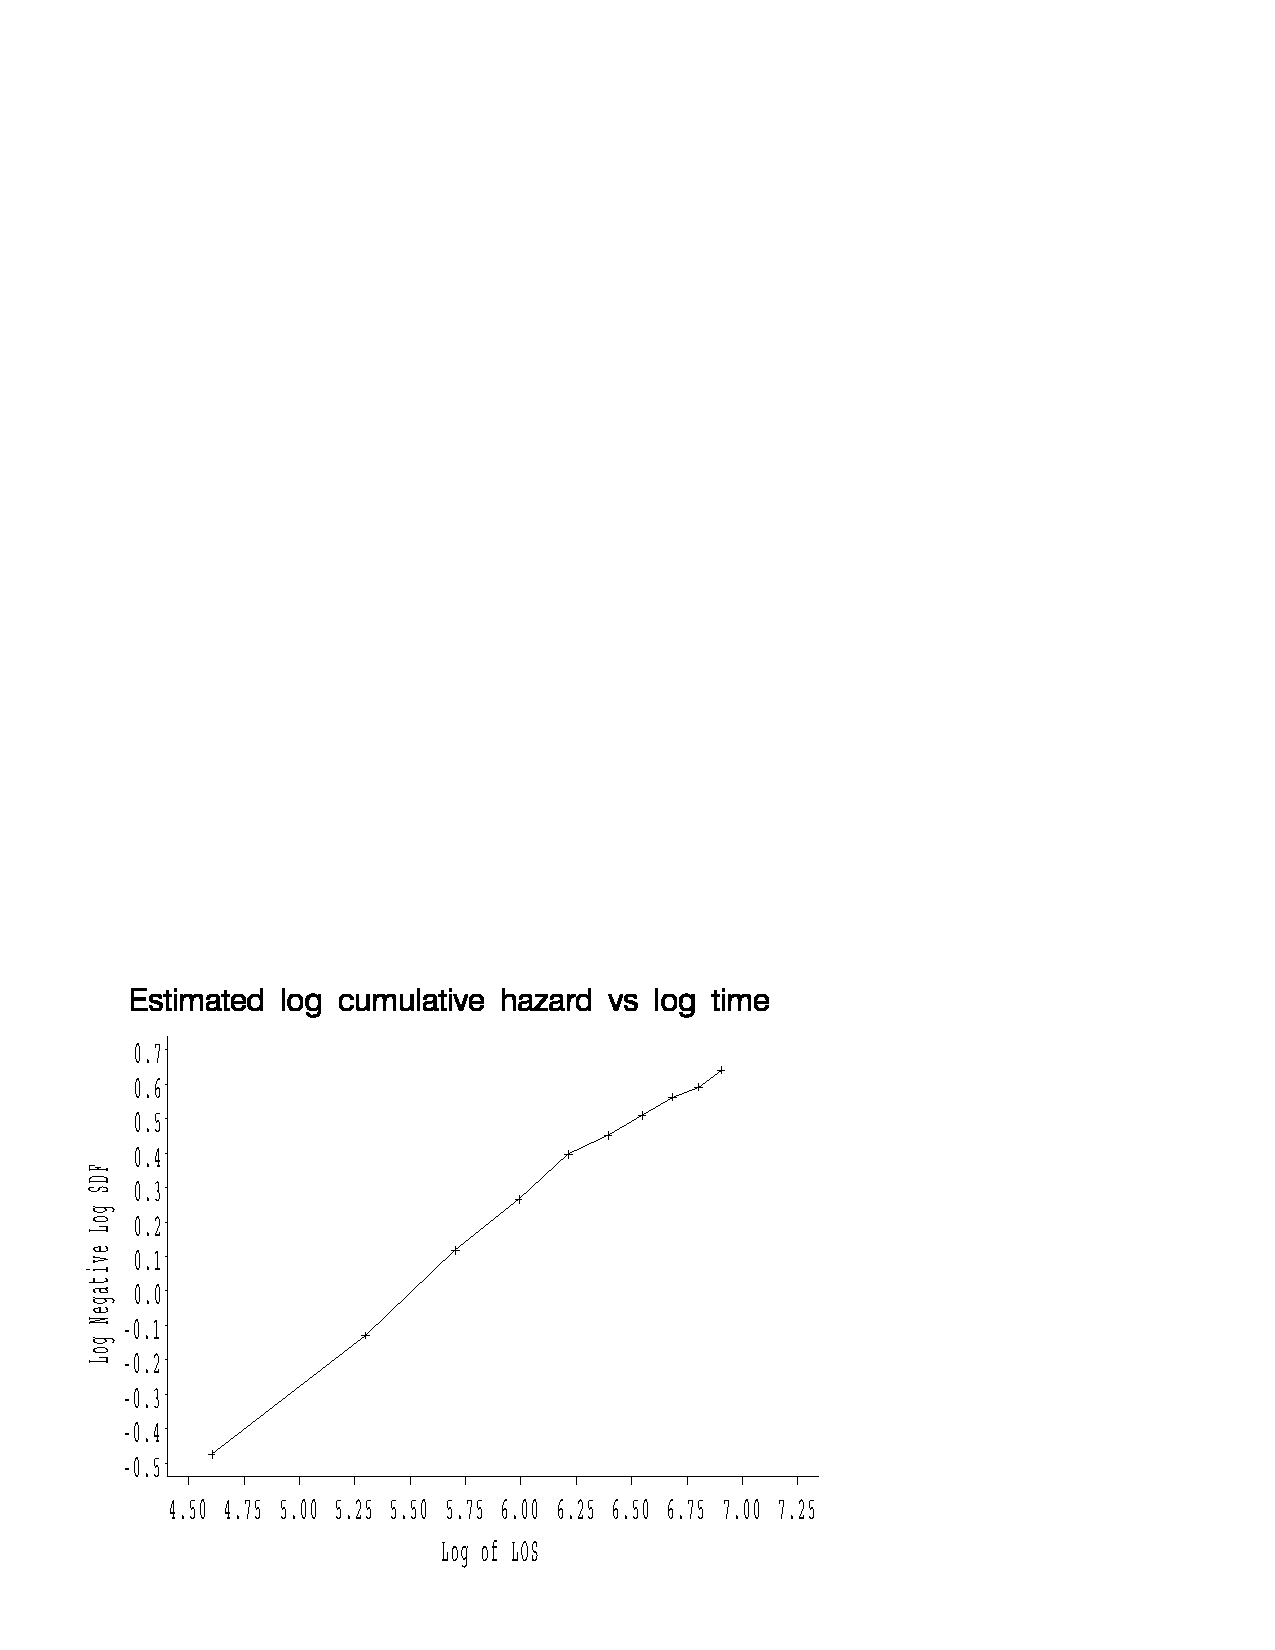
\includegraphics[width=3in]{nh_lls.pdf}}
\end{frame} 
\begin{frame}{Comparison of methods for the two-sample problem}

\underline{\bf Data:}

\begin{center}
\begin{tabular}{lcccc}
\hline
& $Z_i$ & Subjects & Events & Follow-up \\ \hline
{\bf Group 0:}~~
& $Z_{i}= 0$ & $n_0$ & $d_0$ & $t_0=\sum_{i=1}^{n_0} X_i$\\[1ex]
{\bf Group 1:}
& $Z_{i}= 1$ & $n_1$ & $d_1$ & $t_1=\sum_{i=1}^{n_1} X_i$ \\ \hline
\end{tabular}
\end{center}

\vspace{0.1in}
{\bf In General:}
\begin{eqnarray*}
\lambda_z(t) & = & \lambda(t,Z=z) ~~~~~~~\mbox{for } z=0 ~\mbox{or}~ 1.
\end{eqnarray*}
The hazard rate depends on the value of the covariate $Z$.  In this case,
we are assuming that we only have a single covariate,  and it is
binary ($Z=1$ or $Z=0$)

\end{frame}
\begin{frame}{ Reading from Collett}

Reference (Collett):
\\[2ex]
\begin{tabular}{ll}
{\bf Section(s)} & {\bf Description} \\ \hline
4.1.1, 4.1.2 & Exponential properties\\
4.1.3 & Weibull properties\\
4.3.1, 4.4.2 & Exponential ML estimation\\
4.3.2 & Weibull ML estimation\\
4.5 & General Weibull regression\\
4.6 & Model selection - Weibull regression\\
4.7 & Weibull/AFT model connection\\
Ch.6 & AFT - Other parametric models\\
\end{tabular}
%%%%%%%%%%%%%%%%%%%%%%%%%%%%%%%%%%%%%%%%%%%%%%%%%%%%%%%%%%%%%%%%
\end{frame} 
\begin{frame}{ Models}

\underline{\bf Exponential Regression:}
\begin{eqnarray*}
\lambda_z(t) & = & \exp(\beta_0 + \beta_1 Z)\\[3ex]
\Rightarrow \lambda_0 & = & \exp(\beta_0)\\[1ex]
            \lambda_1 & = & \exp(\beta_0+\beta_1)\\[1ex]
                   HR & = & \exp(\beta_1)
\end{eqnarray*}

\underline{\bf Weibull Regression:}
\begin{eqnarray*}
\lambda_z(t) & = & \kappa ~\exp(\beta_0 + \beta_1 Z) ~t^{\kappa-1}\\[3ex]
\Rightarrow \lambda_0 & = & \kappa ~\exp(\beta_0) ~t^{\kappa-1}\\[1ex]
            \lambda_1 & = & \kappa ~\exp(\beta_0+\beta_1) ~t^{\kappa-1}\\[1ex]
                   HR & = & \exp(\beta_1)
\end{eqnarray*}
\end{frame}
\begin{frame}{Models (cont'd)}
\underline{\bf Proportional Hazards Model:}
\begin{eqnarray*}
\lambda_z(t) & = & \lambda_0(t) \exp(\beta_1)\\[3ex]
\Rightarrow \lambda_0 & = & \lambda_0(t) \hspace{1.5in} \mbox{KM?}\\[1ex]
            \lambda_1 & = & \lambda_0(t) \exp(\beta_1)\\[1ex]
                   HR & = & \exp(\beta_1)
\end{eqnarray*}
%%%%%%%%%%%%%%%%%%%%%%%%%%%%%%%%%%%%%%%%%%%%%%%%%%%%%%%%%%%%%%%%
\end{frame} 
\begin{frame}{Remarks}
We make the following remarks:
\begin{itemize}
\item Exponential model is a special case of the Weibull model
with $\kappa=1$ (note: Collett uses $\gamma$ instead of $\kappa$)

\item Exponential and Weibull models are both special cases of the Cox
PH model.

{\bf How can you show this?}
\item If either the exponential model or the Weibull model is valid,
then these models will tend to be more efficient than PH (smaller
s.e.'s of estimates).  This is because they assume a particular
form for $\lambda_0(t)$, rather than estimating it at every death
time.
\end{itemize}
%%%%%%%%%%%%%%%%%%%%%%%%%%%%%%%%%%%%%%%%%%%%%%%%%%%%%%%%%%%%%%%%
\end{frame} 
\begin{frame}{Exponential regression}
For the Exponential model, the hazards are constant over time, given
the value of the covariate $Z_i$:
\begin{eqnarray*}
Z_i=0 \Rightarrow~~~
\hat\lambda_0 & = & \exp(\hat\beta_0)\\[1ex]
Z_i=1 \Rightarrow~~~
\hat\lambda_0 & = & \exp(\hat\beta_0+\hat\beta_1)
\end{eqnarray*}

For the Weibull model, we have to estimate the hazard as a
function of time, given the estimates of $\beta_0, \beta_1$ and $\kappa$:
\begin{eqnarray*}
Z_i=0 \Rightarrow~~~
\hat\lambda_0(t) & = & \hat\kappa ~\exp(\hat\beta_0) ~t^{\hat\kappa-1}\\[1ex]
Z_i=1 \Rightarrow~~~
\hat\lambda_1(t) & = & \hat\kappa ~\exp(\hat\beta_0+\hat\beta_1)
~t^{\hat\kappa-1}
\end{eqnarray*}
However, the ratio of the hazards is still just $\exp(\hat\beta_1)$,
since the other terms cancel out.
\end{frame} 
\begin{frame}{Estimated hazards for the nursing home data}

{\bf Here's what the estimated hazards look like for the
nursing home data:}

\centerline{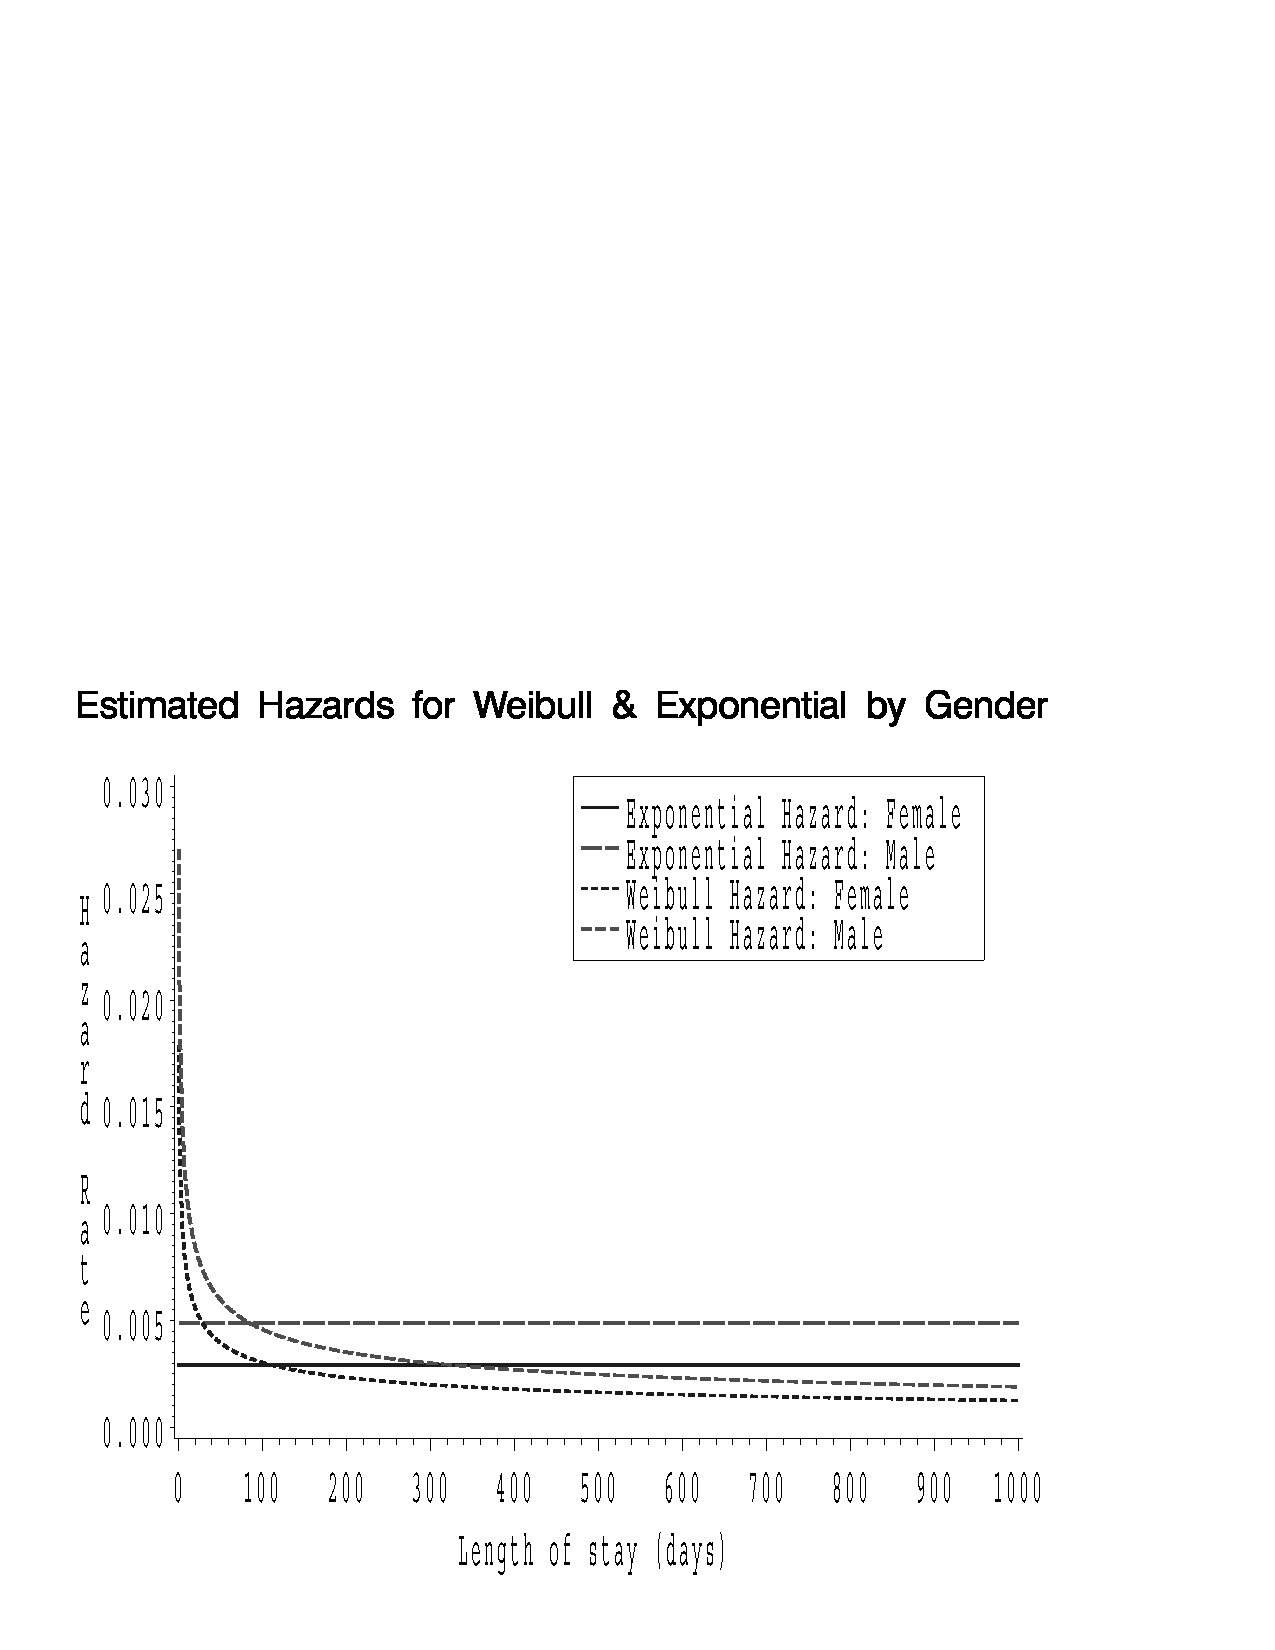
\includegraphics[width=3in]{weibhaz.pdf}}
%%%%%%%%%%%%%%%%%%%%%%%%%%%%%%%%%%%%%%%%%%%%%%%%%%%%%%%%%%%%%%%%
\end{frame} 
\begin{frame}{ Proportional Hazards Model}
To get the MLE's for this model, we have to maximize the Cox partial
likelihood iteratively.  There are not closed form expressions like above.

\begin{eqnarray*}
L(\bfbeta) & = & \prod_{i=1}^{n}
\left[ \frac {e^{\bfbeta {\bfZ}_i }} {\sum_{\ell \in {\cal R}(X_i)}
    e^{\bfbeta {\bfZ}_\ell}} \right]^{\delta_i}\\[4ex]
& = & \prod_{i=1}^{n}
\left[ \frac {e^{\beta_0 + \beta_1 Z_i }} {\sum_{\ell \in {\cal R}(X_i)}
    e^{\beta_0 + \beta_1 Z_\ell}} \right]^{\delta_i}
\end{eqnarray*}
%%%%%%%%%%%%%%%%%%%%%%%%%%%%%%%%%%%%%%%%%%%%%%%%%%%%%%%%%%%%%%%%
\end{frame} 
\begin{frame}[fragile]{ Comparison with Proportional Hazards Model}

\scriptsize
\begin{verbatim}
Call:
coxph(formula = Surv(losyr, fail) ~ gender, data = nurshome)

  n= 1591, number of events= 1269

         coef exp(coef) se(coef)     z Pr(>|z|)
gender 0.3958    1.4855   0.0621 6.373 1.85e-10 ***
---
Signif. codes:  0 ‘***’ 0.001 ‘**’ 0.01 ‘*’ 0.05 ‘.’ 0.1 ‘ ’ 1

       exp(coef) exp(-coef) lower .95 upper .95
gender     1.486     0.6732     1.315     1.678

Concordance= 0.541  (se = 0.006 )
Rsquare= 0.024   (max possible= 1 )
Likelihood ratio test= 38.29  on 1 df,   p=6.11e-10
Wald test            = 40.62  on 1 df,   p=1.852e-10
Score (logrank) test = 41.14  on 1 df,   p=1.415e-10
\end{verbatim}
\normalsize
For the PH model, $\hat\beta_1=0.394$ and $\widehat{HR}=e^{0.394}=1.483$.
%%%%%%%%%%%%%%%%%%%%%%%%%%%%%%%%%%%%%%%%%%%%%%%%%%%%%%%%%%%%%%%%
\end{frame} 
\begin{frame}[fragile]{Comparison with the Logrank test}

\scriptsize
\begin{verbatim}
Call:
survdiff(formula = Surv(losyr, fail) ~ gender, data = nurshome)

            N Observed Expected (O-E)^2/E (O-E)^2/V
gender=0 1173      902      995      8.76      41.1
gender=1  418      367      274     31.88      41.1

 Chisq= 41.1  on 1 degrees of freedom, p= 1.46e-10
 \end{verbatim}
\end{frame} 
\begin{frame}[fragile]{Comparison with the Wilcoxon test}
Note that this is fit by adding {\tt rho=1} in R:
\scriptsize
\begin{verbatim}
Call:
survdiff(formula = Surv(losyr, fail) ~ gender, data = nurshome,
    rho = 1)

            N Observed Expected (O-E)^2/E (O-E)^2/V
gender=0 1173      529      592      6.66      41.8
gender=1  418      236      173     22.73      41.8

 Chisq= 41.8  on 1 degrees of freedom, p= 9.94e-11 
 \end{verbatim}
%%%%%%%%%%%%%%%%%%%%%%%%%%%%%%%%%%%%%%%%%%%%%%%%%%%%%%%%%%%%%%%%
\end{frame} 
\begin{frame}[fragile]{Comparison of HRs and test statistics for effect of {\tt gender}}

\scriptsize
\begin{center}
\begin{tabular}{lcccccc}
\hline       &             &             &    &         &    & Wald\\
Model/Method & $\lambda_0$ & $\lambda_1$ & HR & log(HR) & se(log HR)
& Statistic\\ \hline \\
{\bf Exponential}
& 0.0029 & 0.0049 & 1.676 & 0.5162 & 0.0619 & 69.507 \\[1ex]
{\bf Weibull}\\
~$t=50$  & 0.0040 & 0.0060 & 1.513 & 0.4138 & 0.0636 & 42.381 \\
~$t=100$ & 0.0030 & 0.0046 & 1.513 \\
~$t=500$ & 0.0016 & 0.0025 & 1.513 \\[1ex]
{\bf Logrank}
&         &         &       &        &        & 41.085 \\[1ex]
{\bf Wilcoxon}
&         &         &       &        &        & 41.468 \\[1ex]
\fbox{\bf Cox PH} \\
Ties=Breslow
&         &         & 1.483 & 0.3944 & 0.0621 & 40.327 \\
Ties=Discrete
&         &         & 1.487 & 0.3969 & 0.0623 & 40.565 \\
Ties=Efron
&         &         & 1.486 & 0.3958 & 0.0621 & 40.616 \\
Ties=Exact
&         &         & 1.486 & 0.3958 & 0.0621 & 40.617 \\
Score (Discrete)
&         &         &       &        &        & 41.085\\ \hline
\end{tabular}
\end{center}

%%%%%%%%%%%%%%%%%%%%%%%%%%%%%%%%%%%%%%%%%%%%%%%%%%%%%%%%%%%%%%%%
\end{frame} 
\begin{frame}{Comparison of Mean and Median Survival Times by Gender}

\small
\begin{center}
\begin{tabular}{lccccc}
\hline
             & \multicolumn{2}{c}{Mean Survival} & ~~&
             \multicolumn{2}{c}{Median Survival}\\ \cline{2-3} \cline{5-6}
Model/Method & Female & Male & & Female & Male\\ \hline \\
{\bf Exponential}
& 344.5 & 205.6 & & 238.8 & 142.5 \\[1ex]
{\bf Weibull}
& 461.6 & 235.4 & & 174.2 & 88.8 \\[1ex]
{\bf Kaplan-Meier}
& 318.6 & 200.7 & & 144 & 70 \\[1ex]
{\bf Cox PH}
&       &       & & 131 & 72 \\
(Kalbfleisch/Prentice)
\\ \hline
\end{tabular}
\end{center}
%%%%%%%%%%%%%%%%%%%%%%%%%%%%%%%%%%%%%%%%%%%%%%%%%%%%%%%%%%%%%%%%
\end{frame} 
\end{document}
\begin{frame}{
\normalsize
\begin{center}
{\bf The Accelerated Failure Time Model}
\end{center}
The general form of an accelerated failure time (AFT) model is:
\[ \log(T_i) = \bfbeta_{AFT} \bfZ_i + \sigma \epsilon \]
where
\begin{itemize}
\item $\log(T_i)$ is the log of a survival time
\item $\bfbeta_{AFT}$ is the vector of AFT model parameters
corresponding to the covariate vector $\bfZ_i$
\item $\epsilon$ is a random ``error'' term
\item $\sigma$ is a scale factor
\end{itemize}
{\ \bf In other words, we can model the log-survival times as a linear
function of the covariates!}

The {\tt streg}
command in {\sc stata} (without the exponential or weibull option)
uses this ``log-linear'' model for fitting parametric models.
%%%%%%%%%%%%%%%%%%%%%%%%%%%%%%%%%%%%%%%%%%%%%%%%%%%%%%%%%%%%%%%%
\end{frame} \begin{frame}{
\
By choosing different distributions for $\epsilon$, we can obtain
different parametric distributions:
\begin{itemize}
\item Exponential
\item Weibull
\item Gamma
\item Log-logistic
\item Normal
\item Lognormal
\end{itemize}

We can compare the predicted survival under any of these parametric
distributions to the KM estimated survival to see which one seems to
fit best.

Once we decide on a certain class of model (say, Gamma), we can
evaluate the contributions of covariates by finding the MLE's,
and constructing Wald, Score, or LR tests of the covariate effects.
%%%%%%%%%%%%%%%%%%%%%%%%%%%%%%%%%%%%%%%%%%%%%%%%%%%%%%%%%%%%%%%%
\end{frame} \begin{frame}{
\

We can motivate the AFT model by first demonstrating the following two
relationships:

{\bf 1. For the Exponential Model:}\\[1ex]
If the failure times $T_i=T(\bfZ_i)$ follow an exponential
distribution, i.e., $S_i(t)=e^{-\lambda_i t}$ with
$\lambda_i=exp(\bfbeta \bfZ_i)$, then
\begin{eqnarray*}
\log(T_i) &= & - \bfbeta \bfZ_i + \epsilon
\end{eqnarray*}
where $\epsilon$ follows an extreme value distribution (which just
means that $e^{\epsilon}$ follows a unit exponential distribution).

\end{frame} \begin{frame}{
{\bf 2. For the Weibull Model:}\\[1ex]
If the failure times $T_i=T(\bfZ_i)$ follow a Weibull
distribution, i.e., $S_i(t)=e^{\lambda_i t^{\kappa}}$ with
$\lambda_i=exp(\bfbeta \bfZ_i)$, then
\begin{eqnarray*}
\log(T_i) &= & - \sigma \bfbeta \bfZ_i + \sigma \epsilon
\end{eqnarray*}
where $\epsilon$ again follows an extreme value distribution,
and $\sigma=1/\kappa$.

In other words, both the Exponential and Weibull model can be
written in the form of a log-linear model for the survival times, if
we choose the right distribution for $\epsilon$.
%%%%%%%%%%%%%%%%%%%%%%%%%%%%%%%%%%%%%%%%%%%%%%%%%%%%%%%%%%%%%%%%
\end{frame} \begin{frame}{
\
The log-linear form for the exponential can be derived by:
\begin{itemize}
\item[(1)] Creating a new variable $T_0= T_Z \times \exp(\bfbeta \bfZ_i)$
\item[(2)] Taking the log of $T_Z$, yielding $\log(T_Z) =
\log\left(\frac{T_0}{\exp(\bfbeta \bfZ_i)}\right)$
\end{itemize}

\underline{\bf Step (1):} For an exponential model, recall that:\\
$$S_i(t) = Pr(T_Z \ge t) = e^{- \lambda t},
\mbox{~~~with~} \lambda=\exp(\bfbeta \bfZ_i)$$

It follows that $T_0 \sim exp(1)$:
\begin{eqnarray*}
S_0(t) = Pr(T_0 \ge t) & = & Pr(T_Z \cdot \exp(\bfbeta \bfZ) \ge t)\\[1ex]
& = & Pr(T_Z \ge t \exp(- \bfbeta \bfZ))\\[1ex]
& = & \exp\left[-\lambda ~ t~ \exp(-\bfbeta \bfZ)\right]\\
& = & \exp\left[-\exp(\bfbeta \bfZ)~ t~ \exp(-\bfbeta \bfZ)\right]\\
& = & \exp(-t)
\end{eqnarray*}

\underline{\bf Step (2):} Now take the log of the survival time:
\begin{eqnarray*}
\log(T_Z) & = & \log\left(\frac{T_0}{\exp(\bfbeta\bfZ_i)} \right)\\[1ex]
          & = & \log(T_0) - \log\left(\exp(\bfbeta\bfZ_i)\right)\\[1ex]
          & = & - \bfbeta\bfZ_i + log(T_0)\\[1ex]
          & = & - \bfbeta\bfZ_i + \epsilon
\end{eqnarray*}
where  $\epsilon=\log(T_0)$ follows the {\bf extreme value}
distribution.
%%%%%%%%%%%%%%%%%%%%%%%%%%%%%%%%%%%%%%%%%%%%%%%%%%%%%%%%%%%%%%%%
\end{frame} \begin{frame}{
{\bf Relationship between Exponential and Weibull}

If $T_Z$ has a Weibull distribution, i.e., $S(t) = e^{- \lambda t^\kappa}$\\
with $\lambda=\exp(\bfbeta\bfZ_i)$, then you can show that the new variable

\[ T_Z^* =  T_Z^\kappa\]

follows an exponential distribution with parameter
$\exp(\bfbeta\bfZ_i)$.  Based on the previous page, we can therefore write:
\[ \log(T^*) = -\bfbeta \bfZ  +  \epsilon   \]

(where $\epsilon$ has an extreme value distribution.)\\

But since $\log(T^*) = \log(T^\kappa) = \kappa \times  \log(T)$, we
can write:
\begin{eqnarray*}
 \log(T) & = & \log(T^*)/\kappa \\[2ex]
         & = & (1/\kappa) \left( - \bfbeta \bfZ_i  + \epsilon \right)\\[2ex]
         & = & - \sigma \bfbeta \bfZ_i + \sigma \epsilon
\end{eqnarray*}

where $\sigma=1/\kappa$.
%%%%%%%%%%%%%%%%%%%%%%%%%%%%%%%%%%%%%%%%%%%%%%%%%%%%%%%%%%%%%%%%
\end{frame} \begin{frame}{
\
This motivates the following general definition of the\\
\underline{\bf Accelerated Failure Time Model} by:

\[ \log(T_i) = \bfbeta_{AFT} \bfZ_i + \sigma \epsilon \]

where $\epsilon$ is a random ``error'' term, $\sigma$ is a scale
factor, Y is the log of a survival random variable, and
$$\bfbeta_{AFT} = - \sigma \bfbeta_e$$
where $\bfbeta_e$ came from the hazard $\lambda=\exp(\bfbeta \bfZ)$.

\end{frame} \begin{frame}{
\
{\bf The defining feature of an AFT model is:}

\[    S(t; {\bfZ}) =  S_i(t) = S_0(\phi ~t)  \]

That is, the effect of covariates is to accelerate (stretch) or
decelerate (shrink) the time-scale.

\vspace{0.3in}
{\bf Effect of AFT on hazard:}
\begin{eqnarray*}
\lambda_i(t) & = & \phi ~\lambda_0(\phi t)
\end{eqnarray*}
%%%%%%%%%%%%%%%%%%%%%%%%%%%%%%%%%%%%%%%%%%%%%%%%%%%%%%%%%%%%%%%%
\end{frame} \begin{frame}{
\
One way to interpret the AFT model is via its effect on median
survival times.  If $S_i(t)=0.5$, then $S_0(\phi t)=0.5$.  This means:
\begin{eqnarray*}
M_i & = & \phi M_0
\end{eqnarray*}

\underline{\bf Interpretation:}
\begin{itemize}
\item For $\phi<1$, there is an acceleration of the endpoint\\
(if $M_0=2$yrs in control and $\phi=0.5$, then $M_i=1$yr.
\item For $\phi>1$, there is a stretching or delay in endpoint
\item In general, the lifetime of individual $i$ is $\phi$ times what
they would have experienced in the reference group
\end{itemize}

Since $\phi$ must be positive and a function of the covariates,
we model $\phi=\exp(\bfbeta\bfZ_i)$.
%%%%%%%%%%%%%%%%%%%%%%%%%%%%%%%%%%%%%%%%%%%%%%%%%%%%%%%%%%%%%%%%
\end{frame} \begin{frame}{
{\bf When does Proportional hazards = AFT?}

According to the proportional hazards model:
\[S(t)=S_0(t)^{\exp(\bfbeta\bfZ_i)} \]
and according to the accelerated failure time model:
\[S(t)=S_0(t \exp(\bfbeta \bfZ_i))\]

\vspace{0.1in}
Say $T_i \sim Weibull(\lambda,\kappa)$.  Then
$\lambda(t) = \lambda \kappa t^{(\kappa-1)}$

Under the AFT model:
\begin{eqnarray*}
\lambda_i(t) & = & \phi ~\lambda_0 (\phi t)\\[2ex]
& = & e^{\bfbeta\bfZ_i} ~\lambda_0(e^{\bfbeta\bfZ_i} t)\\[2ex]
& = & e^{\bfbeta\bfZ_i} ~\lambda_0 \kappa \left(e^{\bfbeta\bfZ_i}
t\right)^{(\kappa-1)}\\
& = & \left(e^{\bfbeta\bfZ_i}\right)^{\kappa} ~
\lambda_0 \kappa t^{(\kappa-1)}\\
& = & \left(e^{\bfbeta\bfZ_i}\right)^{\kappa} ~\lambda_0(t)
\end{eqnarray*}

But this looks just like the PH model:
\begin{eqnarray*}
\lambda_i(t) & = & \exp(\bfbeta^*\bfZ_i) ~\lambda_0(t)
\end{eqnarray*}

It turns out that the Weibull distribution (and exponential, since
this is just a special case of a Weibull with $\kappa=1$) is the
only one for which the accelerated failure time and proportional
hazards models coincide.
%%%%%%%%%%%%%%%%%%%%%%%%%%%%%%%%%%%%%%%%%%%%%%%%%%%%%%%%%%%%%%%%
\end{frame} \begin{frame}{
{\bf Special cases of AFT models}
\begin{itemize}
\item Exponential regression:  $\sigma=1$, $\epsilon$ following the
extreme value distribution.
\item Weibull regression:  $\sigma$ arbitrary, $\epsilon$ following the
extreme value distribution.
\item Lognormal regression:   $\sigma$ arbitrary, $\epsilon$ following the
normal distribution.
\end{itemize}

\end{frame} \begin{frame}{
{\bf Examples in stata:}
Using the {\sc streg} command, one has the following options
of distributions for the log-survival times:

\begin{verbatim}
. streg trt, dist(lognormal)
\end{verbatim}

\begin{itemize}
\item exponential
\item weibull
\item gompertz
\item lognormal
\item loglogistic
\item gamma
\end{itemize}
%%%%%%%%%%%%%%%%%%%%%%%%%%%%%%%%%%%%%%%%%%%%%%%%%%%%%%%%%%%%%%%%
\end{frame} \begin{frame}{
\scriptsize
\begin{verbatim}
. streg gender, dist(exponential) nohr
------------------------------------------------------------------------------
      _t |      Coef.   Std. Err.       z     P>|z|       [95% Conf. Interval]
---------+--------------------------------------------------------------------
  gender |    .516186   .0619148      8.337   0.000       .3948352    .6375368
------------------------------------------------------------------------------

. streg gender, dist(weibull) nohr
------------------------------------------------------------------------------
      _t |      Coef.   Std. Err.       z     P>|z|       [95% Conf. Interval]
---------+--------------------------------------------------------------------
  gender |   .4138082   .0621021      6.663   0.000       .2920903    .5355261
     1/p |   1.627501   .0377726                          1.555127    1.703243
------------------------------------------------------------------------------

. streg gender, dist(lognormal)
------------------------------------------------------------------------------
      _t |      Coef.   Std. Err.       z     P>|z|       [95% Conf. Interval]
---------+--------------------------------------------------------------------
  gender |  -.6743434   .1127352     -5.982   0.000      -.8953002   -.4533866
   _cons |   4.957636   .0588939     84.179   0.000       4.842206    5.073066
   sigma |    1.94718    .040584                           1.86924    2.028371
------------------------------------------------------------------------------

. streg gender, dist(gamma)
------------------------------------------------------------------------------
      _t |      Coef.   Std. Err.       z     P>|z|       [95% Conf. Interval]
---------+--------------------------------------------------------------------
  gender |  -.6508469   .1147116     -5.674   0.000      -.8756774   -.4260163
   _cons |   4.788114   .1020906     46.901   0.000        4.58802    4.988208
   sigma |    1.97998   .0429379                          1.897586    2.065951
------------------------------------------------------------------------------
\end{verbatim}
\normalsize
This gives a good idea of the sensitivity of the test of gender to the
choice of model.  It is also easy to get predicted survival curves
under any of the parametric models using the following:
\begin{verbatim}
. streg gender, dist(gamma)
. stcurv, survival
\end{verbatim}
The options {\sc hazard} and {\sc cumhaz} can also be substituted
for {\sc survival} above to obtain plots.
\end{slide}
\end{document}
